% !TeX program = xelatex
% 中文审读稿：与英文正文内容一致，不限制页数。
\makeatletter\def\input@path{{./}{template/}}\makeatother
\PassOptionsToPackage{no-math}{fontspec}
\documentclass[a4paper,12pt,review]{cas-sc}
\geometry{a4paper}
\usepackage[UTF8,scheme=plain,fontset=windows]{ctex}
\usepackage[numbers,sort&compress]{natbib}
\usepackage{bm,algorithm,algpseudocode,placeins}
\renewcommand{\figurename}{图}
\renewcommand{\tablename}{表}
\renewcommand{\abstractname}{摘要}
\renewcommand{\refname}{参考文献}
\floatname{algorithm}{算法}
\newcommand{\R}{\mathbb R}
\newcommand{\C}{\mathbb C}
\newcommand{\Rea}{\operatorname{Re}}
\begin{document}
\let\WriteBookmarks\relax
\shorttitle{宽带直接定位的变量投影曲率更新}
\shortauthors{B. Hao et al.}
\title[mode=title]{未知宽带源直接定位中Newton精修的变量投影曲率更新}
%% Author 1: Benjian Hao
\author[inst1]{Benjian Hao}[orcid=0000-0002-6676-7306]
\ead{bjhao@xidian.edu.cn}
% TODO(CRediT): Add \credit{...} after all authors approve their roles.
%% Author 2: Xinlei Wang
\author[inst1]{Xinlei Wang}[orcid=0000-0002-6855-3686]
\ead{wangxinlei@stu.xidian.edu.cn}
% TODO(CRediT): Add \credit{...} after all authors approve their roles.
%% Author 3: Zan Li (corresponding author)
\author[inst1]{Zan Li}[orcid=0000-0002-5207-6504]
\cormark[1]
\ead{zanli@xidian.edu.cn}
% TODO(CRediT): Add \credit{...} after all authors approve their roles.
\cortext[cor1]{Corresponding author.}
\affiliation[inst1]{organization={State Key Laboratory of Integrated Service Networks, School of Telecommunications Engineering, Xidian University},
  city={Xi'an},
  postcode={710071},
  country={China}}
% 资助及其他未确认信息按要求留空。
\begin{abstract}
在直接位置确定中，未知宽带波形使源位置与大量频域系数相互耦合。块Newton正交匹配追踪降低了搜索维数，但固定系数的位置更新可能进展缓慢，即使接受试探位置时已经重新估计波形。本文针对这一局部精修过程构造变量投影曲率更新。消去当前源系数后，位置Hessian中去除了一个半正定耦合项；局部分析解释了该项为何可能拖慢收敛。曲率按频率累计，只需计算小矩阵。在240条双源观测的配对实验中，两版使用相同的波形消元接受目标，采用消元曲率使平均完整耗时降低83.77\%，20 m门槛下的成功／失败判定逐例一致，终态联合拟合与驻点指标均未恶化。另用480条新源位置观测检验完整流程，区分局部效率收益与逐源定位的构型敏感性。该方法保留基于残差的源发现机制，提高了块精修的计算效率。
\end{abstract}
\begin{keywords}
直接位置确定\sep 变量投影\sep Newton精修\sep 未知波形\sep 块正交匹配追踪
\end{keywords}
\maketitle

\section{引言}
直接位置确定（DPD）联合拟合同步接收站的观测以估计辐射源位置，省去了中间时延的关联步骤\cite{ChenHudsonYao2002,WeissAmar2005}。当未知波形频谱重叠时，需要同时估计位置和频域系数。逐源发现降低了空间搜索规模，但反复进行的局部精修可能成为主要计算开销。

Newton正交匹配追踪（NOMP）结合了源发现、Newton精修和循环反馈\cite{Mamandipoor2016}。它在发现阶段估计增益，在精修过程中更新增益，并通过联合最小二乘重新拟合全部增益；但计算Newton方向时，仍将当前增益视为固定参数。多频块NOMP将这一结构推广到二维位置和逐频未知源系数\cite{Yang2022}，其固定系数位置导数是本文最直接的精修参照。QNOMP在基于导频的信道估计中，通过联合准Newton精修和增益重估更新时延与角度\cite{Zeng2025}。

本文保留块NOMP的源发现和循环更新，将最优波形系数随位置的变化纳入Newton曲率。基于经典变量投影\cite{GolubPereyra1973}，推导宽带DPD响应的显式逐频修正，并分析位置与波形耦合导致缓慢局部更新的原因。小矩阵累加使单步计算量仍随频点数线性增长。受控实验采用相同的波形消元接受目标及数值保护，以分离曲率选择对后续迭代和完整耗时的影响。本文贡献在于这一块精修构造及其机制验证，而非增益重估本身。

\section{模型与局部目标}
记$\bm r_l\in\R^2$和$\bm p_k\in\Omega\subset\R^2$分别为第$l$个接收站和第$k$个源的位置。对于$L$个同步单天线站及已知源数$K$，保留的DFT观测满足
\begin{equation}
 \bm x_f=\sum_{k=1}^K\bm a_f(\bm p_k)s_{k,f}+\bm n_f,
 \qquad [\bm a_f(\bm p)]_l=\frac{\exp[-\mathrm j2\pi f d_l(\bm p)/c_0]}{d_l(\bm p)},
 \label{eq:model}
\end{equation}
其中$d_l(\bm p)=\|\bm p-\bm r_l\|$，$c_0$为传播速度，$f\in\mathcal F$为有正负之分的基带频率，$F=|\mathcal F|$。未知系数$s_{k,f}\in\C$包含发射功率。已知相对幅度遵循自由空间损耗规律，与波长有关的公共系数并入$s_{k,f}$\cite{ITURP5252024}。本文采用静态、已标定的直达基带时延模型，不含射频载波相位或随机链路增益。公共观测窗近似忽略了站间记录边缘的差别\cite{ChenHudsonYao2002}。独立复高斯采样噪声的方差为$\sigma_t^2$；对长度$N$的记录采用$1/N$归一化DFT后，保留频点的噪声方差仍为$\sigma_t^2/N$。数值计算将距离下限设为1 m，以下光滑导数适用于该保护区之外。

令$E=\sum_f\|\bm x_f\|^2>0$。精修第$j$个源时，固定其余源的拟合贡献，构造$\bm y_f=\bm x_f-\sum_{k\ne j}\bm a_f(\bm p_k)\widehat s_{k,f}$。对于试探位置$\bm z\in\R^2$，有
\begin{align}
 \mathcal L(\bm z,\bm q)&=E^{-1}\sum_f\|\bm y_f-\bm a_f(\bm z)q_f\|^2,
 &\widehat q_f(\bm z)&=\frac{\bm a_f^H\bm y_f}{\bm a_f^H\bm a_f},\label{eq:ls}\\
 \phi(\bm z)&=\min_{\bm q}\mathcal L(\bm z,\bm q)
 =E^{-1}\sum_f\left(\|\bm y_f\|^2-\frac{|\bm a_f^H\bm y_f|^2}{\bm a_f^H\bm a_f}\right).
 \label{eq:profile}
\end{align}
其中$\bm x_f,\bm y_f,\bm n_f\in\C^L$，$\bm q\in\C^F$。上标$H$和$T$分别表示共轭转置和普通转置，$\mathrm j^2=-1$，$I_2$为单位矩阵。该局部调用消去了当前源的全部频域系数，其余源的拟合贡献保持固定。

\section{波形消元曲率}
在当前位置取$q_f=\widehat q_f$，令$\bm e_f=\bm y_f-\bm a_fq_f$，并定义$\bm a_{f,i}=\partial\bm a_f/\partial z_i$与$\bm a_{f,ij}=\partial^2\bm a_f/\partial z_i\partial z_j$。固定系数求导得到
\begin{align}
 g_i&=-\frac{2}{E}\Rea\sum_f\bm e_f^H\bm a_{f,i}q_f,\label{eq:g}\\*
 [H_{zz}]_{ij}&=\frac{2}{E}\Rea\sum_f
 \left(|q_f|^2\bm a_{f,i}^H\bm a_{f,j}-\bm e_f^H\bm a_{f,ij}q_f\right).
 \label{eq:hfixed}
\end{align}
由于系数已处于最优值，$\bm g$同时也是$\phi$的梯度，但$H_{zz}$并非$\phi$的Hessian。将各频点系数的实部和虚部组成$\bm u\in\R^{2F}$，对$\nabla_u\mathcal L(\bm z,\widehat{\bm u}(\bm z))=0$求导，可得
\begin{equation}
 \frac{\partial\widehat{\bm u}}{\partial\bm z}=-H_{uu}^{-1}H_{uz},\qquad
 H_{\rm VP}=H_{zz}-H_{zu}H_{uu}^{-1}H_{uz}.
 \label{eq:schur}
\end{equation}
这里$H_{\rm VP}$是条件局部目标$\phi$的Hessian：仅消去当前源的系数，其余源的拟合贡献保持固定；它不是全部源系数联合消元后的位置目标的Hessian。该消元恒等式\cite{GolubPereyra1973}要求响应光滑、系数最优解在局部唯一。各Hessian块均在当前系数最优值处计算。这里$H_{uu}$为分块对角矩阵，其逐频$2\times2$块为$2\|\bm a_f\|^2 I_2/E$，因而正定。因此$H_{zz}-H_{\rm VP}\succeq0$：固定系数曲率包含了可由波形调整补偿的响应变化。

为显式计算修正项，令$\bm D_f=[\bm a_{f,1},\bm a_{f,2}]$、$\bm c_f=q_f(\bm a_f^H\bm D_f)^T$及$\bm b_f=(\bm e_f^H\bm D_f)^T$。频率$f$对应的混合块为
\begin{equation}
 H_{zu,f}=\frac{2}{E}
 [\Rea(\bm c_f-\bm b_f),\ \operatorname{Im}(\bm c_f+\bm b_f)].
 \label{eq:cross}
\end{equation}
逐频累加其Schur修正即可避免构造稠密的$2F\times2F$矩阵。记$\bm v_l=(\bm z-\bm r_l)/d_l$、$b_l=-d_l^{-1}-\mathrm j2\pi f/c_0$，响应导数为
\begin{equation}
 \nabla a_{fl}=a_{fl}b_l\bm v_l,\qquad
 \nabla^2a_{fl}=a_{fl}\left[(b_l^2+d_l^{-2})\bm v_l\bm v_l^T
 +\frac{b_l}{d_l}(I_2-\bm v_l\bm v_l^T)\right].
 \label{eq:response}
\end{equation}
两种曲率的单次局部计算量均为$\mathcal O(FL)$。预期收益来自更新次数和循环次数减少，而非频点复杂度阶数降低。两者均采用式\eqref{eq:model}中未归一化的响应。

局部收敛关系进一步说明了这种差别。在内部极小点$\bm z^*$处，假设$H_{zz}^*$和$H_{\rm VP}^*$均正定。记误差$\bm\epsilon=\bm z-\bm z^*$，对$\phi$采用完整的固定曲率更新，其线性化为
\begin{equation}
 \bm\epsilon^+=\left[I_2-(H_{zz}^*)^{-1}H_{\rm VP}^*\right]\bm\epsilon
 +o(\|\bm\epsilon\|).
 \label{eq:rate}
\end{equation}
迭代矩阵的特征值位于$[0,1)$；当消元曲率相对固定曲率很小时，特征值接近1。精确消元Newton曲率则消除了这一线性项。这解释了强耦合下的缓慢局部进展，实际耗时还取决于回溯及外层源更新。

算法\ref{alg:vp}将该更新用于块NOMP。源发现对当前残差$\bm r_f$扫描网格，最大化$\sum_f|\bm a_f^H\bm r_f|^2/\|\bm a_f\|^2$。局部调用求解$(H_{\rm VP}+\lambda I_2)\bm d=-\bm g$，其中$\lambda$使最小特征值满足给定下限；有界回溯只接受不增大$\phi$的试探位置。接受的块更新和联合系数拟合均不增加残差能量，因此目标值序列收敛，但不保证位置达到全局最优。
\begin{algorithm}[htbp]
\caption{已知源数$K$的VP-BNOMP}\label{alg:vp}
\begin{algorithmic}[1]
\State 初始化空源集合和残差$\bm r_f=\bm x_f$。
\For{$k=1,\ldots,K$}
\State 从网格发现位置，按梯度式\eqref{eq:g}、曲率式\eqref{eq:hfixed}--\eqref{eq:response}及接受目标式\eqref{eq:profile}精修，减去拟合贡献。
\Repeat
\State 逐源将其贡献加回残差，执行相同局部精修并更新残差。
\Until{循环能量变化达到阈值或触及安全上限}
\State 通过最小二乘联合重估全部源系数，并更新残差。
\EndFor
\State 输出源位置。
\end{algorithmic}
\end{algorithm}

\FloatBarrier
\section{实验}
采用独立BPSK波形和根升余弦成形，符号率10 Mbaud、滚降系数0.25、脉冲支撑区间为$\pm10$个符号，其余设置见表\ref{tab:settings}。固定噪声与弱源，仅调整另一源的功率。带内SNR定义为四站平均孤立信号功率与$\sigma_t^2B/f_s$之比，功率差按平均接收功率计算。0 dB时保持源身份，不重新排序。每组配对采用相同IQ和初始化规则。以总平方距离最小完成一次位置匹配，两个匹配误差均不超过20 m时判定成功。
\begin{table}[pos=H]
\caption{共同仿真与精修参数。}\label{tab:settings}
\centering
\begin{tabular}{ll}
\toprule
项目 & 设置 \\
\midrule
站点坐标（m）；源数 & $(500,0),(0,500),(-500,0),(0,-500)$；$K=2$ \\
采样率；记录长度 & $f_s=50$ MHz；$N=8192$ \\
信号；处理频带 & 零中心；$B=12.5$ MHz；$|f|\le7$ MHz \\
弱源带内SNR；功率差 & 6 dB；$0,3,6,9,12,15$ dB \\
搜索区域；初始网格 & $[-1000,1000]^2$ m；20 m \\
局部步数；特征值下限 & 最多5步；$10^{-9}$ \\
步长上限；局部退出 & 50 m；接受位移$<0.01$ m \\
回溯因子 & $1,1/2,1/4,1/8,1/16$ \\
循环停止；安全上限 & 归一化能量变化$\le10^{-8}$；10,000轮 \\
\bottomrule
\end{tabular}
\end{table}

\subsection{受控曲率比较}
曲率对照使用20个固定源位置构型，每构型两次波形／噪声实现、六档功率差，共240条观测。双源均在站内、任一源在站外及双源均在站外四类各占五个构型。位置从$[-950,950]^2$ m均匀抽样，并要求源间距至少300 m，距站点至少150 m，距中心至少100 m，距任意站点对所在直线至少50 m；筛选只使用几何条件。

FC--VP和VP--VP名称的前半部分表示方向所用曲率，后半部分表示试探接受目标。FC--VP采用式\eqref{eq:hfixed}的固定系数曲率；VP--VP采用式\eqref{eq:schur}的消元曲率，即本文提出的VP-BNOMP。两者均用式\eqref{eq:profile}接受试探，在每个试探位置重估系数，共用源发现与联合重估时序，以及表\ref{tab:settings}的参数。FC--VP是适用于当前模型的受控参照，并非某篇论文实现的原样复现。

运行环境为Windows、Python 3.10、PyTorch 2.8、双精度、RTX 4070 Ti SUPER和20个CPU线程。完整耗时包含DFT、带限、传输、搜索、精修、轨迹记录及最终检查，并同步GPU；预热和磁盘读写不计入。配对中的全部运行均按共同循环能量规则停止，该规则不要求最终联合梯度精度相同。

\begin{table}[pos=H]
\caption{定位表现与完整耗时。$e_s,e_w$为强／弱源RMSE（m）；$\bar t,t_{50},t_{95}$为平均、中位及P95耗时（s）。两个分组使用不同观测。}\label{tab:results}
\centering
\begin{tabular}{lrrrrrr}
\toprule
方法 & 成功数 & $e_s$ & $e_w$ & $\bar t$ & $t_{50}$ & $t_{95}$ \\
\midrule
\multicolumn{7}{l}{A. 曲率配对（$n=240$）}\\
FC--VP & 228/240 & 0.906 & 89.706 & 5.574 & 2.836 & 16.161 \\
VP--VP & 228/240 & 0.875 & 86.177 & 0.905 & 0.567 & 2.538 \\
\midrule
\multicolumn{7}{l}{B. 新源位置构型（$n=480$）}\\
AP1 & 480/480 & 0.958 & 2.194 & 0.461 & 0.456 & 0.545 \\
AP5 & 480/480 & 0.958 & 2.194 & 0.906 & 0.893 & 1.078 \\
VP-BNOMP & 390/480 & 202.882 & 206.261 & 1.051 & 0.629 & 4.245 \\
\bottomrule
\end{tabular}
\end{table}

表\ref{tab:results}A显示，消元曲率降低了计算成本，并保持相近的定位表现。两版在相同228条观测上成功，在相同12条上失败。平均完整耗时降低83.77\%，按$1-\bar t_{\rm VP}/\bar t_{\rm FC}$计算，而非逐条降时百分比的平均值。在各固定构型内对随机实现配对重采样，并将同一实现的六档功率差一起保留，4,000次重采样给出的95\%区间为[81.73\%,85.58\%]。该区间以所测构型为条件。

\begin{figure}[pos=H]
\centering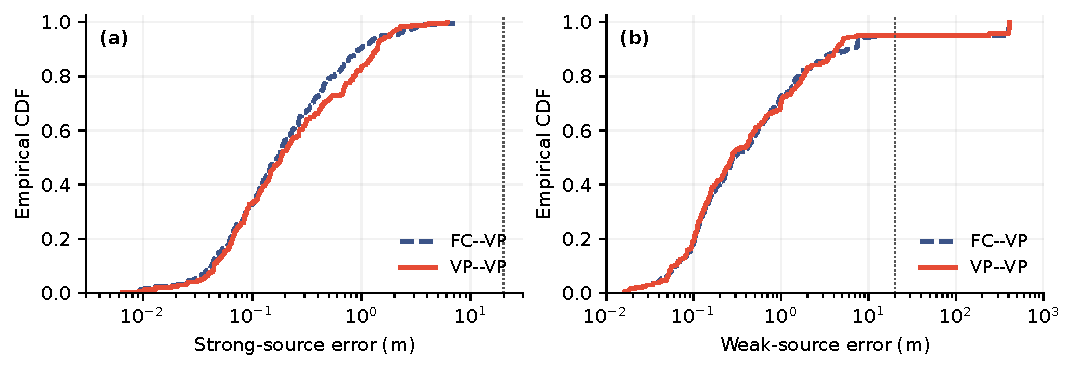
\includegraphics[width=\linewidth]{figures/error_cdf.pdf}
\caption{全部240组曲率配对的匹配误差经验CDF。虚点线标出20 m，对数横轴覆盖完整误差范围。}\label{fig:errors}
\end{figure}

图\ref{fig:errors}中的误差分布相近，包括弱源误差长尾。成功判定一致并不意味着估计位置完全相同，两版的强、弱源RMSE仍有小幅差别。CDF和RMSE均保留全部观测。

\begin{figure}[pos=H]
\centering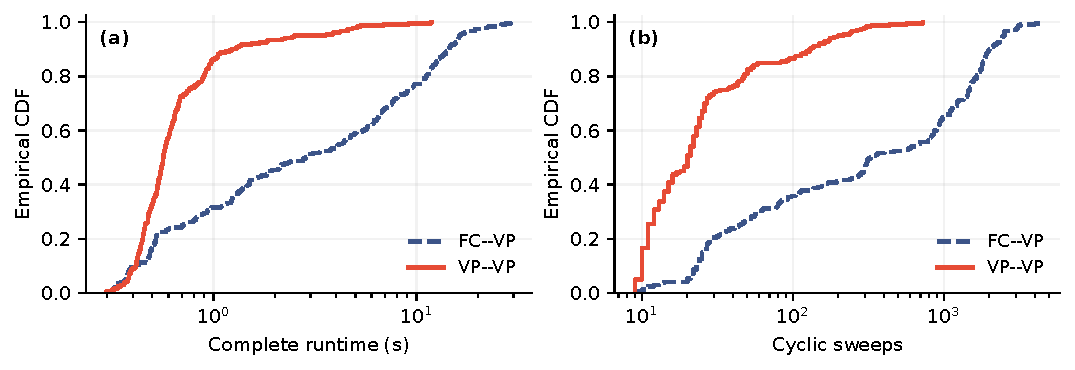
\includegraphics[width=\linewidth]{figures/cost_cdf.pdf}
\caption{同一240组配对的完整耗时及循环次数CDF。循环数统计包含全部源添加阶段。}\label{fig:cost}
\end{figure}

图\ref{fig:cost}显示了慢样本尾部的缩短。平均Newton试探次数由1498.82降至135.55，循环次数由810.90降至47.97；未被接受的方向也计入统计。VP--VP在170/240条观测中更快，平均收益尤其来自慢案例的改善。记录与最终检查的平均开销分别为0.0254/0.0059 s，远小于4.669 s的耗时差。更新与循环次数的减少支持式\eqref{eq:rate}所解释的曲率作用。

\newpage
用同一个完整联合目标检查终态质量：
\begin{equation}
 J(\bm P)=E^{-1}\sum_f\|(I_L-\bm A_f\bm A_f^\dagger)\bm x_f\|^2,
 \quad \bm A_f=[\bm a_f(\bm p_1),\ldots,\bm a_f(\bm p_K)],
 \label{eq:joint}
\end{equation}
其中$\bm P$汇集全部源坐标，$\dagger$表示伪逆。在以米为单位的坐标下，将下边界处的正梯度分量、上边界处的负梯度分量置零，得到箱约束投影梯度，并报告其无穷范数。VP--VP在全部配对中的$J$均不高于FC--VP：199条降低超过$10^{-10}$，41条差值落在该数值容差内。投影梯度的中位数由$2.03\times10^{-6}$降至$1.30\times10^{-7}$，P95由$5.33\times10^{-6}$降至$1.79\times10^{-6}$，且逐例均更小。因此，在共同能量停止规则下，计算节省未伴随终态拟合或驻点指标的恶化。这些指标不证明全局最优，也不替代定位误差。

\subsection{小步机制诊断}
正式轨迹进一步说明了迭代机制。对每条观测，以位移不足0.01 m的已接受更新数除以全部已接受更新数，拒绝更新不计入。该比例的中位数在FC--VP和VP--VP中分别为67.48\%和65.74\%。两版均常见小步，与共同的局部退出阈值一致；小步比例本身不足以解释提速。FC--VP的359,717次试探全部被接受，未触发Hessian修正、步长封顶、回溯缩步或边界裁剪，其小步来自计算所得方向。加入第二源后的循环次数中位数由89.5降至19，P95由1647降至197.85。因此，收益体现为重复循环精修减少，而非步长普遍增大。所有比例均先按观测计算，再作汇总。

已有8条开发观测由四个构型、一次实现和0/15 dB功率差组成，采用计算方向与试探接受时均固定系数、接受后再重估系数的FC--FC参照。21,436次被接受的更新中，17,935次（83.67\%）不足0.01 m，同样没有触发上述四类保护。该独立诊断也说明小步来自计算方向，不与正式配对合并统计。

\FloatBarrier
\subsection{完整定位流程检验}
将测试前已冻结的方法用于16个新源位置构型，每构型五次实现和相同六档功率差，共480条观测，接收站坐标不变。交替投影参照AP1/AP5分别保留条件投影响应评分的一个／五个峰。对每对位置，联合消去两源系数，以完整双源残差作连续联合精修，再返回最终残差最小的位置对；两者的投影梯度阈值均为$10^{-8}$。

表\ref{tab:results}B显示，两版AP全部成功，VP-BNOMP成功率为81.25\%。VP的90条失败集中在四个构型，并已出现在首次保存的完整双源输出中。该输出位于初始源发现和精修之后，不能据此区分哪个阶段造成了失败。这说明降低局部精修成本尚不足以消除逐源定位流程中的构型相关失败。

\begin{samepage}
\section{结论}
波形消元从块Newton曲率中去除了可被系数调整补偿的位置—系数耦合。所得逐频更新保留了基于残差的源发现，减少了重复循环精修。在共同接受和停止规则下，240条观测的配对比较节省了83.77\%的平均完整耗时，20 m成功判定逐例一致，误差分布相近，终态联合拟合与驻点指标均未恶化。新源位置测试表明，改善局部曲率尚不足以消除完整逐源定位流程中的构型相关失败，源发现与精修之间的相互作用仍值得进一步研究。
\end{samepage}

% 资助及其他未经确认的声明按要求留空。
\bibliographystyle{template/cas-model2-names}
\bibliography{references/references}
\end{document}
